\chapter{Conclusion and Future Work}
\label{chap:conclusion}

In this document, we first started Chapter \ref{chap:introduction} with motivational and problem statement followed by research objectives of this work. In Chapter \ref{chap:fundamentals}, the fundamental concepts from existing literature has been provided in a detailed way. In Chapter \ref{chap:motivatingScenario}, a motivating scenario has been taken and explained based on the guidelines and real life scenarios discussed in some previous work. In Chapter \ref{chap:analysis}, a detailed requirements analysis and literature review from the existing approaches has been provided. This is followed by Chapter \ref{chap:approach}, which provides detailed description about the methodology and characteristics of the modeling process. A detailed case study has been provided in Chapter \ref{chap:casestudy}, which helps to explain the abstract concepts discussed in the earlier chapter in a concrete way. This chapter also validates the developed web–based editor by providing examples that satisfies the research objectives discussed in Chapter \ref{chap:introduction} and also conformance of the motivating scenario discussed in Chapter \ref{chap:motivatingScenario} with the developed system.

 \begin{figure}
 	\centering
 	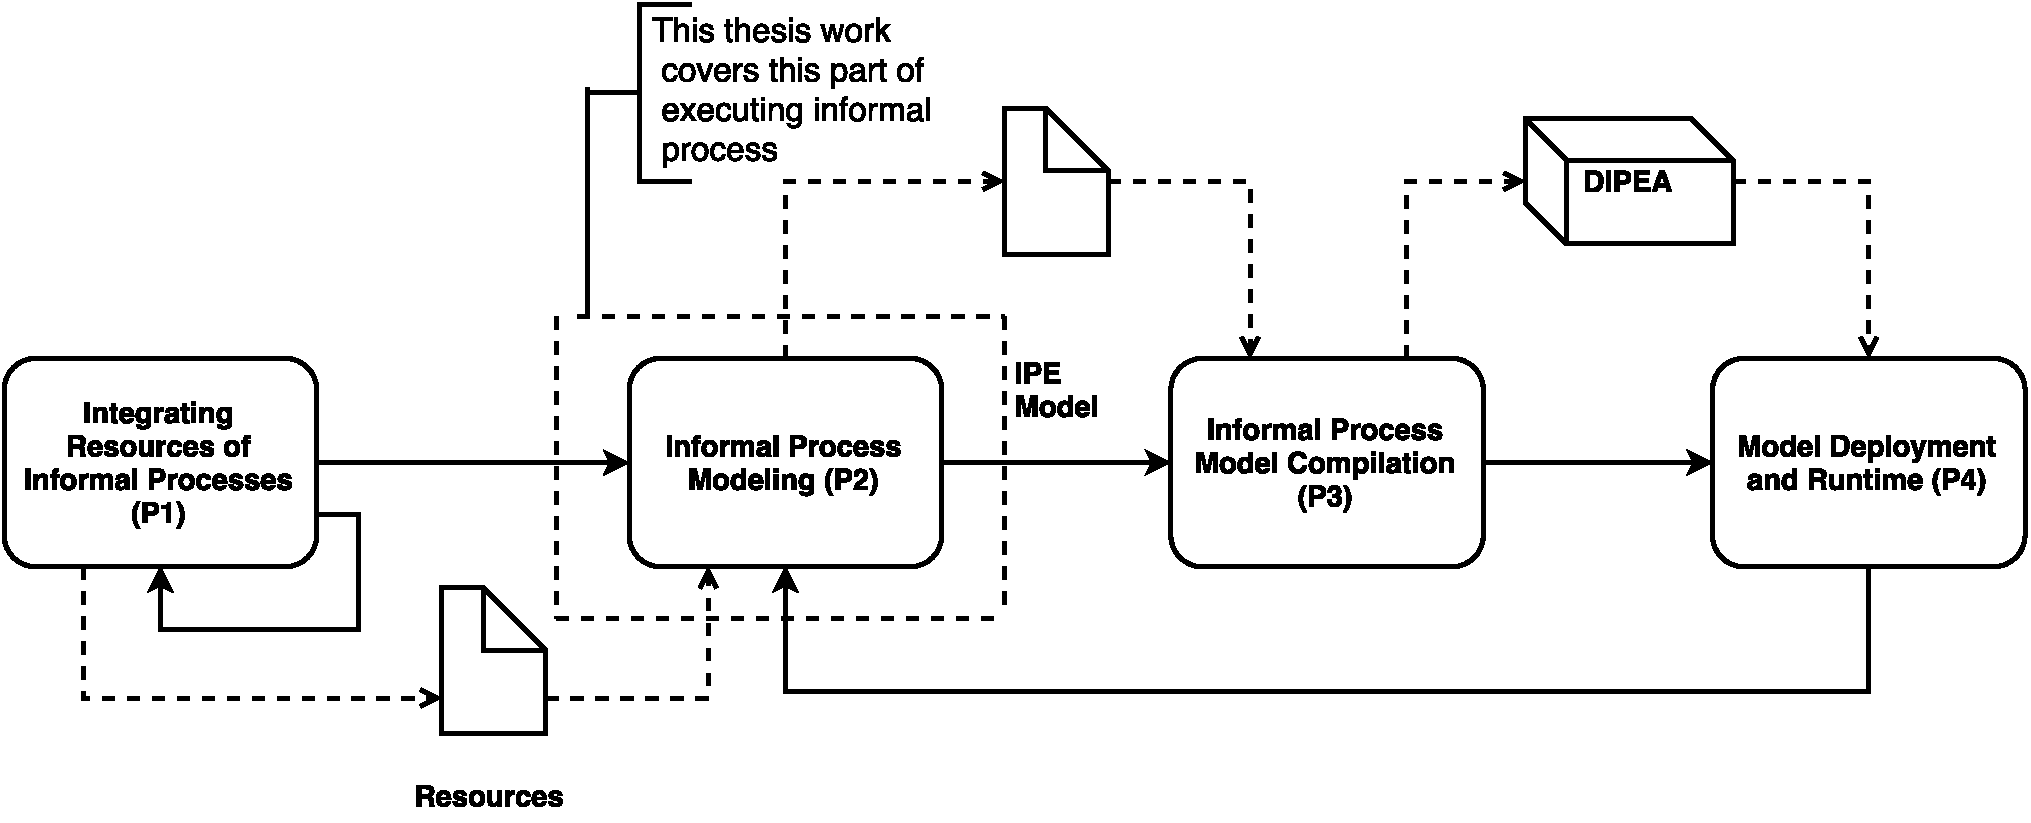
\includegraphics [width= \textwidth]{conclusionimage.pdf}
 	\caption{Contribution of the thesis work}
 	\label{fig:conclusionimage}
 \end{figure}
 
The place of this thesis work in the execution steps of informal process is shown in the Figure \ref{fig:conclusionimage}. The developed editor serves the purpose of creating descriptive models for informal process, intentions, strategies, capabilities, resources and contexts. This created models are used by the next phases of compilation (P3) and execution (P4). This work has not provided details of formal definitions like which execution steps has to be taken by which resources. This work of resource-centric informal process modeling provides complementary \textit{informal} guides and definitions of intentions, strategies, capabilities and resources of a process. 

%%%%%%%%%%%%%%%%%%%%%%%%%%%%%%%%%%%%%%%%%%%%%%%%%%%%%%%%%%%%%%%%%%%%%%%%%
\section*{Future Work}
\label{sec:futurework}
%%%%%%%%%%%%%%%%%%%%%%%%%%%%%%%%%%%%%%%%%%%%%%%%%%%%%%%%%%%%%%%%%%%%%%%%%
Each resources can be related with other resources through \textit{relationships}. This helps business experts to create models with logical resource structures. In this thesis work, we have addressed resource models without relationships and left the ones contain relationships as future work. This is due to the fact that relationships are optional entities in each model and also due to the broad context of this work \cite{Sungur2014a}. 

As discussed in Chapter \ref{chap:introduction}, the web based editor developed as part of this master thesis work, will be further extended such that it can generate deployable entities from the current descriptive information. These deployable entities will be further developed as compilable and executable entities in phases P3 and P4 of the InProXec\cite{Sungur2015}. Also extension of providing mobile support to this web editor are also part of future work. 





